%*********************************************************************
% fduMaththesis: 复旦大学数学科学学院博士毕业论文 LaTeX 模版
% 模版基于开源项目 by 曾祥东(https://github.com/stone-zeng/fduthesis)开发, 
% 部分内容摘自数学科学学院2023年毕业生邹森博士的毕业论文。
% 该模版旨在帮助复旦大学数学科学学院的博士研究生规范撰写毕业论文,符合学院的格式要求。
% 
% 注:
%   1. 请确保使用 UTF-8 编码保存
%   2. 请使用 XeLaTeX 或 LuaLaTeX 编译
%   3. 请阅读说明文档<复旦数学科学学院博士毕业论文LaTeX模版使用说明>,细节设置可参考<源项目说明文档>以及源项目github地址。
%*********************************************************************
\documentclass[type=doctor]{fduthesis}

% !TEX root = ./main.tex

\fdusetup{
	style = {
		% font = times,
		% 西文字体(包括数学字体)
		%   font = garamond|libertinus|lm|palatino|times|times*|none
		%
		% cjk-font = fandol,
		% 中文字体
		%   cjk-font = adobe|fandol|founder|mac|sinotype|sourcehan|windows|none
		font-size = -4,
		hyperlink = none,
		% 超链接样式
		%   hyperlink = border|color|none
		bib-backend = biblatex,
		% 参考文献支持方式
		% 允许选项:
		%   bib-backend = bibtex|biblatex
		bib-resource = {main.bib},
		% 参考文献数据源
		% 可以是单个文件,也可以是用英文逗号 “,” 隔开的一组文件
		% 如果使用 biblatex,则必须明确给出 .bib 后缀名
		bib-style = numerical,
		% 参考文献样式
		% 允许选项:
		%   bib-style = author-year|numerical|<其他样式>
		% 说明:
		%   author-year  著者—出版年制
		%   numerical    顺序编码制
		%   <其他样式>   使用其他 .bst(bibtex)或 .bbx(biblatex)格式文件
		%
		% cite-style = {},
		% 引用样式
		% 默认为空,即与参考文献样式保持一致
		% 仅适用于 biblatex;如要填写,需保证相应的 .cbx 格式文件能被调用
		%
		% declaration-page = {declaration.pdf},
		% 插入扫描版的声明页 PDF 文档
		% 默认使用预定义的声明页,但不带签名
   },
	info = {
		title = {论文题目},
		title* = {English Title},
		author = {某\quad 某},
		author* = {Jane Doe},
		supervisor = {某\quad 某\quad 教~授},
		department = {数学科学学院},
		major = {计算数学},
		degree = academic,
		% 学位类型:
		%   degree = academic|professional
		student-id = {10010101010},
		% date = {2023 年 1 月 1 日},
		% 默认为编译日期
		instructors = {{某\quad 某\quad 教~授},{某\quad 某\quad 教~授},{某某某\quad 教~授}},
		keywords = {关键词1, 关键词2, 关键词3, 关键词4},
		keywords* = {KeyWords1, KeyWords2, KeyWords3, KeyWords4},
		clc = {O24},
	}
}

% 序号
\usepackage{enumerate}

% 定义图片文件目录与扩展名
\graphicspath{{figs/}}
\DeclareGraphicsExtensions{.pdf,.eps,.png,.jpg,.jpeg}

% 子图宏包
\usepackage{subcaption}
\usepackage{bicaption}

% 确定浮动对象的位置,可以使用 [H],强制将浮动对象放到这里(可能效果很差)
\usepackage{float}

% 表格排列
\usepackage{array}

% 固定宽度的表格
\usepackage{tabularx}

% 使用三线表:toprule,midrule,bottomrule。
\usepackage{booktabs}

% 表格中支持跨行
\usepackage{multirow}

% 使用长表格
\usepackage{longtable}

% 附带脚注的表格
\usepackage{threeparttable}

% 附带脚注的长表格
\usepackage{threeparttablex}

% 算法环境宏包
\usepackage[ruled,vlined,linesnumbered]{algorithm2e}
% \usepackage{algorithm, algorithmicx, algpseudocode}

% 代码环境宏包
\usepackage{listings}
\lstdefinestyle{lstStyleCode}{%
  aboveskip         = \medskipamount,
  belowskip         = \medskipamount,
  basicstyle        = \ttfamily\zihao{6},
  commentstyle      = \slshape\color{black!60},
  stringstyle       = \color{green!40!black!100},
  keywordstyle      = \bfseries\color{blue!50!black},
  extendedchars     = false,
  upquote           = true,
  tabsize           = 2,
  showstringspaces  = false,
  xleftmargin       = 1em,
  xrightmargin      = 1em,
  breaklines        = false,
  framexleftmargin  = 1em,
  framexrightmargin = 1em,
  columns           = flexible,
  keepspaces        = true,
  texcl             = true,
  mathescape        = true
}
\lstnewenvironment{codeblock}[1][]{%
  \lstset{style=lstStyleCode,#1}}{}

% 绘图宏包
\usepackage{tikz}
\usetikzlibrary{arrows.meta, shapes.geometric,cd}

% 超链接
\usepackage{xcolor}
\usepackage{hyperref}

% 页码显示
% \usepackage{fancyhdr}
% \pagestyle{fancy}
\fancyfoot{} 
\fancyfoot[EL,OR]{\small\thepage} 
\fancypagestyle{plain}{
    \fancyfoot{}
    \fancyfoot[EL,OR]{\small\thepage} 
}
% `L`, `C`, `R`分别对应左、中、右,`E`, `O`对应偶数页和奇数页


% 自定义引用样式,支持可选参数
\NewDocumentCommand{\mycite}{o m}{%
  \IfNoValueTF{#1}
    {\scalebox{1.2}[1.2]{\raisebox{-0.70ex}{\cite{#2}}}}
    { \scalebox{0.9}[0.9]{\raisebox{0.10ex}{\textnormal{[#1, {\scalebox{1.3}[1.3]{\raisebox{-0.80ex}{\citealp{#2}}}}]}}}}}



\begin{document}

% 前置部分包含目录、中英文摘要以及符号表等
\frontmatter

% 目录
\tableofcontents

% 插图索引
%\listoffigures*
% 表格索引
%\listoftables*
% 算法索引
%\listofalgorithms*

% 插图目录
%\listoffigures

% !TEX root = ../main.tex

\begin{abstract}
  中文摘要
\end{abstract}

\begin{abstract*}
  English abstract
\end{abstract*}


\mainmatter
% 建议采用多文件编译的方式
% 比较好的做法是把每一章放进一个单独的 tex 文件里,并在这里用 \include 导入,例如
%   \include{chapter1}
%   \include{chapter2}
%   \include{chapter3}

\chapter{简介}
复旦大学数学科学学院研究生毕业论文 LaTeX 模版基于开源模版fduthesis开发by 曾祥东\footnote{https://github.com/stone-zeng/fduthesis},我们对他表示感谢。本模板的第一版由复旦大学数学科学学院2021级罗心悦整理完成,目前为迭代的第二版模板,由2019级冯典在第一版的基础上进行了更新。关于模板更新的内容,我们将在下文详细指出。部分内容摘自复旦大学数学科学学院2023年毕业生邹森博士的毕业论文。说明性文字参考了上海交通大学学位论文模版\footnote{https://github.com/sjtug/SJTUThesis}。 

本模板依然在持续的迭代更新中,学院每学年将在官网\footnote{https://math.fudan.edu.cn/c1/39/c30396a639289/page.htm}提供一次大的更新,随时迭代更新的版本请跳转\href{https://github.com/VeMath/fduMath_thesis/tree/v1.0.0}{{\color{red} github仓库}}\footnote{https://github.com/VeMath/fduMath\_thesis/tree/v1.0.0}。
欢迎大家指出模板的不足之处,有任何意见与建议可以在github仓库中提交issue或者联系维护管理员罗心悦:xinyueluo21@m.fudan.edu.cn和张晨阳:24110180062@m.fudan.edu.cn。


该模版旨在帮助复旦大学数学科学学院的研究生规范撰写毕业论文,符合学院的格式要求,更多细节可以参考《复旦数学科学学院研究生毕业论文\LaTeX{}模版使用说明》。

\section{更新说明}
这一节将给出与上一节的差别,其中对于模板本身的更改仅需了解。对于论文书写比较关键的更改,我们将会用{\color{blue} 蓝色}进行标注。
\subsection{关于引用}

事实上,如果使用\textbackslash cite命令,我们将发现引用的上标会出现在文字的右上角,比如文献\cite{ChenPDE}。{\color{blue} 我们在setup.tex文件中对引用命令进行了重写,如有需求,请使用\textbackslash mycite命令,比如文献\mycite{ChenPDE}。}

\textbf{如果有更好的解决办法,欢迎大家与我们联系。}

\subsection{关于页码位置}

第一版中的页码出现在每一页的正下方,我们对此进行了调整,现在的页码位置分奇偶,奇数页出现在右下角,而偶数页出现在左下角。

目前模板默认的方式是奇数页在右下角,偶数页在左下角。如果确实需要修改回居中格式,可在文件setup.tex中进行修改。
只需将setup.tex中对应代码片段的LE,RO更改为C即可。

奇数页右下角,偶数页左下角:
\begin{codeblock}
\fancyfoot [LE,RO] { \thepage }
\fancypagestyle{plain}{
    \fancyhf{}
    \fancyfoot[LE,RO]{\thepage} 
}
\end{codeblock}

页码居中:
\begin{codeblock}
\fancyfoot [C] {  \thepage }
\fancypagestyle{plain}{
    \fancyhf{}
    \fancyfoot[C]{\thepage} 
}
\end{codeblock}

\subsection{关于目录索引颜色}
我们新增了一种超链接的颜色,这使得原先红色的目录及索引,以黑色的形式呈现。


% !TEX root = ../main.tex

\chapter{数学语言}

\section{数学符号和公式}

\begin{itemize}
    \item 公式应另起一行居中排版。公式后应注明编号,按章顺序编排,编号右端对齐。
    \item 公式末尾是需要添加标点符号的,至于用逗号还是句号,取决于公式下面一句是接着公式说的,还是另起一句。
    \begin{equation}
  \frac{2h}{\pi}\int_{0}^{\infty}\frac{\sin\left( \omega\delta \right)}{\omega}
  \cos\left( \omega x \right) \mathrm{d}\omega = 
  \begin{cases}
    h, & \left| x \right| < \delta, \\
    \frac{h}{2}, & x = \pm \delta, \\
    0, & \left| x \right| > \delta.
  \end{cases}
\end{equation}
    \item 公式较长时最好在等号“$=$”处转行。
    \begin{align}
    & I (X_3; X_4) - I (X_3; X_4 \mid X_1) - I (X_3; X_4 \mid X_2) \nonumber \\
  = & [I (X_3; X_4) - I (X_3; X_4 \mid X_1)] - I (X_3; X_4 \mid \tilde{X}_2) \\
  = & I (X_1; X_3; X_4) - I (X_3; X_4 \mid \tilde{X}_2).
\end{align}
\item 公式较长时最好在等号“$=$”处转行。
如果在等号处转行难以实现,也可在 $+$、$-$、$\times$、$\div$ 运算符号处转行,转行
时运算符号仅书写于转行式前,不重复书写。
\begin{multline}
  \frac{1}{2} \Delta (f_{ij} f^{ij}) =
    2 \left(\sum_{i<j} \chi_{ij}(\sigma_{i} - \sigma_{j})^{2}
    + f^{ij} \nabla_{j} \nabla_{i} (\Delta f) \right. \\
  \left. + \nabla_{k} f_{ij} \nabla^{k} f^{ij} +
    f^{ij} f^{k} \left[2\nabla_{i}R_{jk}
    - \nabla_{k} R_{ij} \right] \vphantom{\sum_{i<j}} \right).
\end{multline}
\end{itemize}



\section{定理环境}

这里举一个“定义”和“定理”的例子。

\begin{definition}[非负整指数索伯列夫空间\cite{ChenPDE}]
设$\Omega\subset\mathbb{R}^n$是一个给定区域,令$m$为非负整数,$1\leq p\leq \infty$.定义索伯列夫空间$W^{m,p}$为
$$
W^{m,p}(\Omega)=\left\{u\in L^p(\Omega): \text{对任意}\alpha\in \mathbb{N}_{0}^n\text{满足 }0\leq |\alpha|\leq m, D^{\alpha}u\in L^p(\Omega) \right\},
$$
并装备以范数
\begin{equation*}
\begin{aligned}
\|u\|_{W^{m,p}(\Omega)} &= \left( \sum_{|\alpha|\leq m} \|D^{\alpha}u\|_{L^p(\Omega)}^p \right)^{1/p},\quad 1\leq p <\infty, \label{eq:sobolev-norm}\\
\|u\|_{W^{m,\infty}(\Omega)} &= \max_{|\alpha|\leq m} \|D^{\alpha}u\|_{L^{\infty}(\Omega)}.
\end{aligned}
\end{equation*}
\end{definition}


\begin{theorem}[索伯列夫嵌入定理{\cite{AF2003}}]\label{thm:sobolev-embedding}
令$\Omega$为$\mathbb{R}^n$上一个有$C^{\infty}$光滑边界的有界区域.令$j\geq 0,m\geq 1$为整数,$1\leq p<\infty$,如下嵌入关系成立:
\begin{enumerate}
\item 如果$mp>n>(m-1)p$,则
$$
W^{m,p}(\Omega) \hookrightarrow C^{0,s}(\overline{\Omega}), \quad \text{对于 }0<s\leq m-\frac{n}{p}.
$$
如果$n=(m-1)p$,则
$$
W^{m.p}(\Omega) \hookrightarrow C^{0,s}(\overline{\Omega}), \quad \text{对于 }0<s<1.
$$
\item 如果$1\leq k\leq n$,以及$mp=n$,则
$$
W^{j+m,p}(\Omega)\hookrightarrow W^{j,q}(\Omega), \quad \text{对于 }p\leq q < \infty.
$$
\item 如果$mp<n$,则
$$
W^{j+m,p}(\Omega) \hookrightarrow W^{j,q}(\Omega), \quad \text{对于 }p\leq q \leq p^{*}:=\frac{np}{n-mp}.
$$
\end{enumerate}
\end{theorem}



\section{线性方程的适定性理论}\label{sec:linear-wellposedness}
本节摘自邹森博士的毕业论文,包含一些数学符号的使用、定理的叙述与证明、数学式的引用。

在这一节中,我们讨论线性薛定谔方程
\begin{equation}\label{eq:schrodinger-0}
\left\{\begin{aligned}
-\Delta u - k^2 u +c(x)u &=F, && x\in\Omega,\\
u &=f, && x\in\partial\Omega
\end{aligned}\right.
\end{equation}
弱解的适定性,从而定义反问题的观测数据DtN算子.此外,为研究非线性方程的适定性,我们使用了线性亥姆霍兹方程
\begin{equation}\label{eqn:Helmholtz}
\left\{\begin{aligned}
-\Delta u - k^2 u &=F, && x\in\Omega,\\
u &=f, && x\in\partial\Omega
\end{aligned}\right.
\end{equation}
的强解理论,我们也在本节中加以介绍.这些结论都可以从一般形式椭圆方程的弱解和强解理论导出.为简洁起见,我们首先给出如下定义:我们定义散度型微分算子为
\begin{equation}\label{eq:divergence-form}
L:=-\sum_{i=1}^n D_i(a^{ij}(x)D_{j})+c(x).
\end{equation}
称散度型微分算子$L$在区域$\Omega$上满足椭圆性条件,如果对于任意$x\in\Omega$,$\xi\in\mathbb{R}^n$,存在常数$\lambda,\Lambda>0$,使得
\begin{equation}\label{eq:strict-elliptic}
\lambda |\xi|^2 \leq \sum_{i,j=1}^n a^{ij}(x)\xi_{i}\xi_{j} \leq \Lambda|\xi|^2 .
\end{equation}
另外我们定义非散度型微分算子
\begin{equation}\label{eq:nondivergence-form}
L=-\sum_{i,j=1}^{n}a^{ij}(x)D_{ij} + c(x).
\end{equation}
类似地,对于非散度型微分算子,我们也可以定义其椭圆性条件:对于任意$x\in\Omega$,$\xi\in\mathbb{R}^n$,存在常数$\lambda,\Lambda>0$,使得
\begin{equation*}
\lambda |\xi|^2 \leq \sum_{i,j=1}^n a^{ij}(x)\xi_{i}\xi_{j} \leq \Lambda|\xi|^2 .
\end{equation*}
对于以上两种形式的微分算子,在后文的讨论中,除非特殊说明,我们假定对于$1\leq i,j\leq n$,有$a^{ij}(x)\in C^{\infty}(\overline{\Omega})$以及$c\in L^{\infty}(\Omega)$.

\subsection{弱解的存在性和连续依赖性}\label{sec:weak-solution}

我们首先叙述一般形式椭圆方程的Dirichlet问题弱解的存在性:
\begin{theorem}[Dirichlet问题弱解的存在性{\cite{Chen2elliptic}}]\label{thm:weak-solution}
令$L$为\eqref{eq:divergence-form}中定义的散度型椭圆微分算子,令$\Omega\subset\mathbb{R}^n$为有界开区域,使得Sobolev嵌入定理在其上成立.对于$\mu\in\mathbb{R}$,Dirichlet问题
\begin{equation}\label{eq:dirichlet-equation}
\left\{\begin{aligned}
& Lu+\mu u = F,\\
& u-g\in H_0^1(\Omega)\end{aligned}\right.
\end{equation}
的解有两种情况:
\begin{enumerate}[(1)]
\item 对任意$F\in H^{-1}(\Omega)$,$g\in H^{1}(\Omega)$,\eqref{eq:dirichlet-equation}存在唯一弱解$u\in H^1(\Omega)$;
\item 存在一个非平凡的$u\in H^1_0(\Omega)$使得$Lu+\mu u=0$.
\end{enumerate}
更进一步,满足情形(2)的全体$\mu$构成的集合为可数离散的,$\infty$是唯一可能的极限点,我们称这样的$\mu$为$L$算子在$\Omega$上的Dirichlet特征值,记为$\operatorname{Spec}_{\Omega}(L)$,或者简写为$\operatorname{Spec}(L)$.对于每一Dirichlet特征值$\mu$,其对应的特征函数空间是有限维的.
\end{theorem}

如果增加$c\geq 0$几乎处处成立的假设条件,有如下结论:
\begin{theorem}[Dirichlet问题的$H^1$弱解{\cite{Chen2elliptic}}]\label{thm:regularity}
令$L$为\eqref{eq:divergence-form}中定义的散度型椭圆微分算子,令$\Omega\subset\mathbb{R}^n$为有界开区域,使得其上成立索伯列夫嵌入定理.进一步假设$c\geq 0$几乎处处成立.对于任意$F\in H^{-1}(\Omega)$和$g\in H^1(\Omega)$,Dirichlet问题
\begin{equation}
\left\{\begin{aligned}
&Lu = F, \\
& u-g\in H^{1}_{0}(\Omega)
\end{aligned}\right.
\end{equation}
存在唯一弱解,而且满足估计式
\begin{equation}
\|u\|_{H^1_0(\Omega)} \leq C\left(\|F\|_{H^{-1}(\Omega)} +\|g\|_{H^1(\Omega)} \right),
\end{equation}
其中常数$C$与$F$和$g$无关.
\end{theorem}

在\eqref{eq:schrodinger-0}中我们仅假设$c\in L^{\infty}(\Omega)$,不满足定理\ref{thm:regularity}中$c\geq 0$几乎处处成立的条件,但是通过避开特征值的假设,我们依然可以利用定理\ref{thm:weak-solution}和定理\ref{thm:regularity}得到\eqref{eq:schrodinger-0}弱解的适定性结论:
\begin{corollary}[线性薛定谔方程\eqref{eq:schrodinger-0}的适定性]\label{cor:Schrodinger-weak-solution}
令$\Omega\subset\mathbb{R}^n$为带$C^1$边界的有界开区域.如果$k^2$不是$-\Delta+c$在$\Omega$上的Dirichlet特征值,则对于任意$F\in H^{-1}(\Omega)$,$f\in H^{1/2}(\partial\Omega)$,Dirichlet问题\eqref{eq:schrodinger-0}存在唯一解$u\in H^1(\Omega)$,且满足估计式
\begin{equation}\label{eq:regularity-weak-solution}
\|u\|_{H^1(\Omega)} \leq C\left(\|F\|_{H^{-1}(\Omega)} +\|f\|_{H^{1/2}(\partial\Omega)} \right),
\end{equation}
其中常数$C$仅仅依赖于$k,c$和$\Omega$.
\end{corollary}
注意到当$c(x)\equiv 0$时,上述推论依然成立,因此我们也可以得到\eqref{eqn:Helmholtz}的适定性.

\begin{proof}
根据定理\ref{thm:weak-solution},由于$k^2$不是$-\Delta+c$在$\Omega$上的Dirichlet特征值,故我们可以得到$u$的存在唯一性.现在我们证明弱解$u$满足\eqref{eq:regularity-weak-solution}.不失一般性,我们只考虑齐次边界条件$f=0$的情形.

由于$c\in L^{\infty}(\Omega)$,故存在常数$s\in\mathbb{R}$,使得$c(x)+s\leq 0$对于$x\in\Omega$几乎处处成立.我们记$L:=-\Delta +c$,$L_{s}=-\Delta +s +c$.令定理\ref{thm:regularity}中$g\equiv 0$,我们可以得到$L_{s}$为$H_{0}^1(\Omega)\rightarrow H^{-1}(\Omega)$的有界线性算子,且存在连续的逆算子$L_{s}^{-1}:H^{-1}(\Omega)\rightarrow H^{1}_0(\Omega)$.对于$s$使得$k^2+s\ne 0$,我们记$\sigma=(k^2+s)^{-1}$,则对于$u\in H^{1}_0(\Omega)$有如下等价形式
\begin{equation}\label{eq:eu0}
Lu=k^2 u +F \quad \Leftrightarrow \quad L_{s} u = (k^2+s)j\circ i(u) + F
\quad \Leftrightarrow \quad (\sigma I-K)(i(u)) = \sigma i L_s^{-1}F
\end{equation}
其中$i: H^{1}_0(\Omega)\rightarrow L^2(\Omega)$,$j:L^2(\Omega)\rightarrow H^{-1}(\Omega)$为自然的包含映射,$K:=i\circ L_s^{-1} \circ j$.

由于我们假设$k^2\notin\operatorname{Spec}(-\Delta+c)$,根据定理\ref{thm:regularity}的证明过程,$K$为紧自伴算子{\cite{Chen2elliptic}}.故我们可以取得$s$使得$\sigma\notin\operatorname{Spec}(K)$,此时$\sigma I-K$为$L^2(\Omega)\rightarrow L^2(\Omega)$的可逆线性算子.也就是说,对于任意$F\in H^{-1}(\Omega)$,存在$\tilde{u}\in L^2(\Omega)$,使得
\begin{equation}\label{eq:eu1}
(\sigma I-K)\tilde{u} = \sigma i L_s^{-1}F.
\end{equation}
结合\eqref{eq:eu0}和\eqref{eq:eu1}我们可以得出存在$u\in H^{1}_0(\Omega)$使得$\tilde{u}=i(u)$.根据定理\ref{thm:regularity}以及$\sigma I-K$和$L_{s}$的可逆性,我们有
\begin{equation*}
\begin{aligned}
\|u\|_{H^1(\Omega)} &\leq C\left( \left\|(k^2+s) j(\tilde{u})\right\|_{H^{-1}(\Omega)} + \|F\|_{H^{-1}(\Omega)} \right)\\
&\leq C\left( \|\tilde{u}\|_{L^2(\Omega)} + \|F\|_{H^{-1}(\Omega)} \right)\\
& \leq C\left( \left\|\sigma(\sigma I-K)^{-1}\circ i\circ L^{-1}_s F\right\|_{L^2(\Omega)} + \|F\|_{H^{-1}(\Omega)} \right)\\
& \leq C\|F\|_{H^{-1}(\Omega)}.
\end{aligned}
\end{equation*}

对于非齐次边界条件的情况,即$f\ne 0$,我们可以对$w=u-Ef$应用以上过程得到\eqref{eq:regularity-weak-solution},其中$E$为$\operatorname{Tr}:H^{1}(\Omega)\rightarrow H^{1/2}(\partial\Omega)$的右逆算子.
\end{proof}


% !TeX root = ../main.tex

\chapter{图表}
\section{插图}
插图功能是利用TeX的特定编译程序提供的机制实现的,不同的编译程序支持不同的图形方式。XeTeX支持插入 EPS、PDF、PNG、JPEG 格式的图片。一般图形都是处在浮动环境中。之所以称为浮动是指最终排版效果图形的位置不一定与源文
件中的位置对应。如果要强制固定浮动图形的位置,请使用float宏包,它提供了 \texttt{[H]} 参数。

\subsection{单个图形}
\begin{figure}[H]
    \begin{center}
        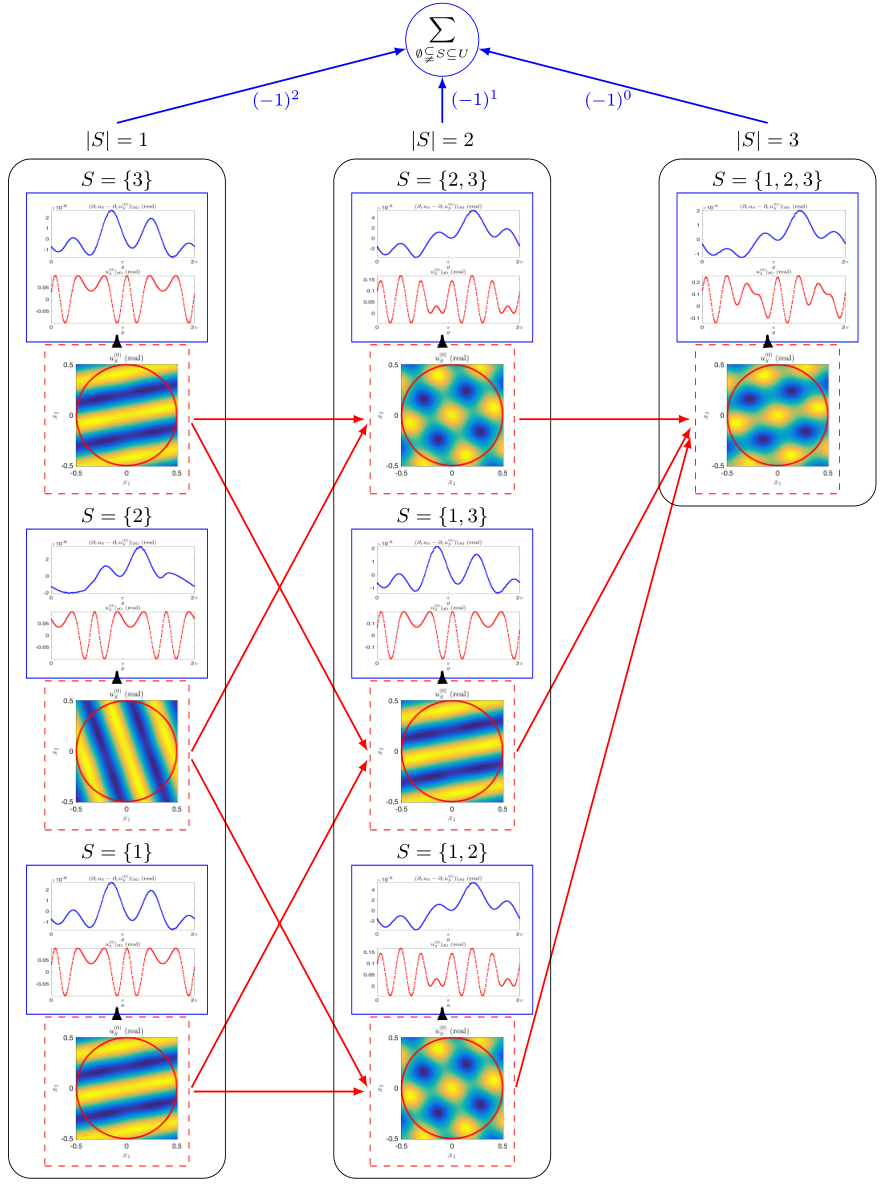
\includegraphics[width=0.5\textwidth]{./figs/cost.png}
\caption[Alessandrini-PIE等式与组合解$u_{S}^{(0)}$]{在非线性次数$m=3$和波数$k=15$时,组合解$u_{S}^{(0)}$的生成.\textbf{红色矩形(虚线)}:$|\xi| = 45.6$时的组合解$u_{S}^{(0)}$.
\textbf{蓝色矩形(实线):} Dirichlet边值 $u_{S}^{(0)} \big|_{\partial\Omega}$ (\textcolor{red}{红色曲线})和线性化Neumann数据的近似$\big( \partial_{\nu} u_{S} - \partial_{\nu} u_{S}^{(0)} \big) \big|_{\partial\Omega}$ (\textcolor{blue}{蓝色曲线}).
\textbf{蓝色圆圈}:根据Alessandrini-PIE等式做组合.}
\label{fig:superposition}
\end{center}
\end{figure}

\subsection{多个图形}
\begin{figure}[H]
\centering
\textbf{非线性次数} $m = 5$ \\[1ex]
\,\hfill \textbf{(i)} $k = 5$ \hfill\,\\
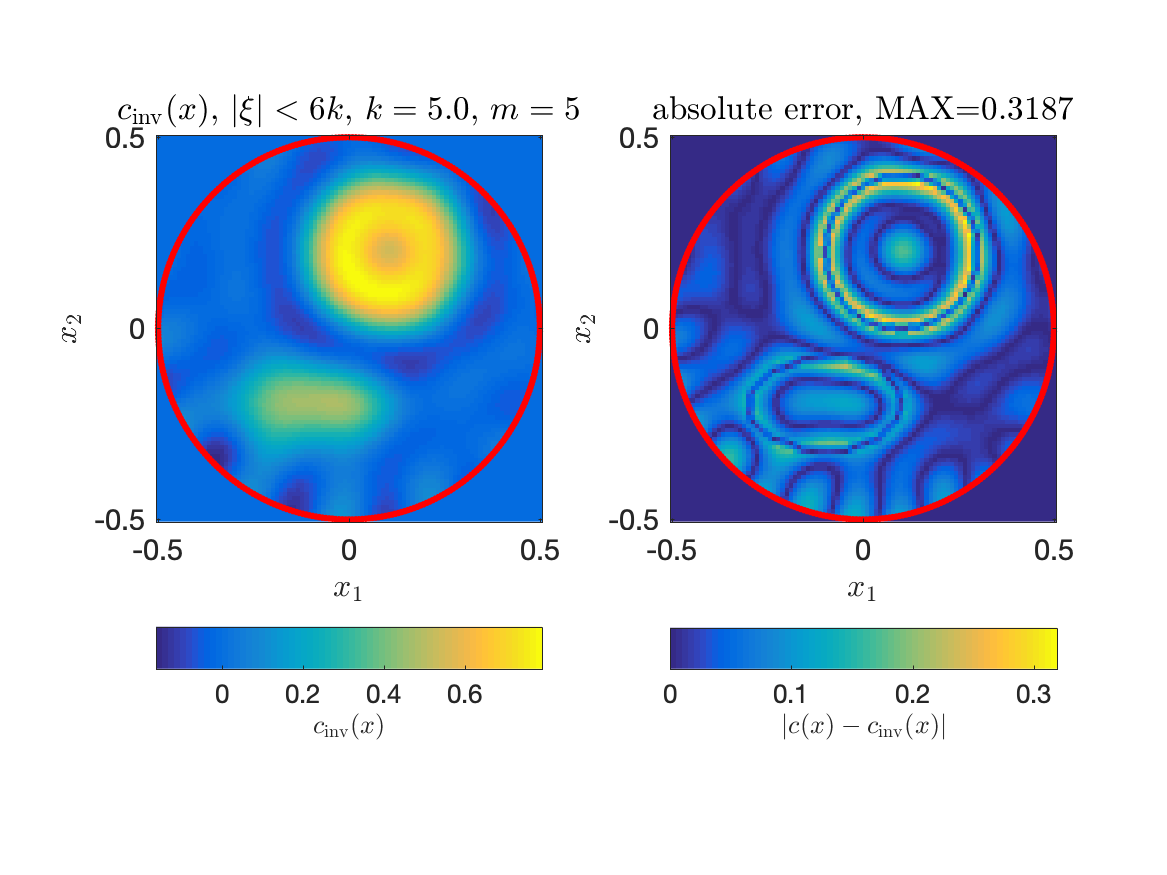
\includegraphics[width=0.45\textwidth,trim=20 60 20 35,clip]{./figs/pwc_5_Ic_0050.png}
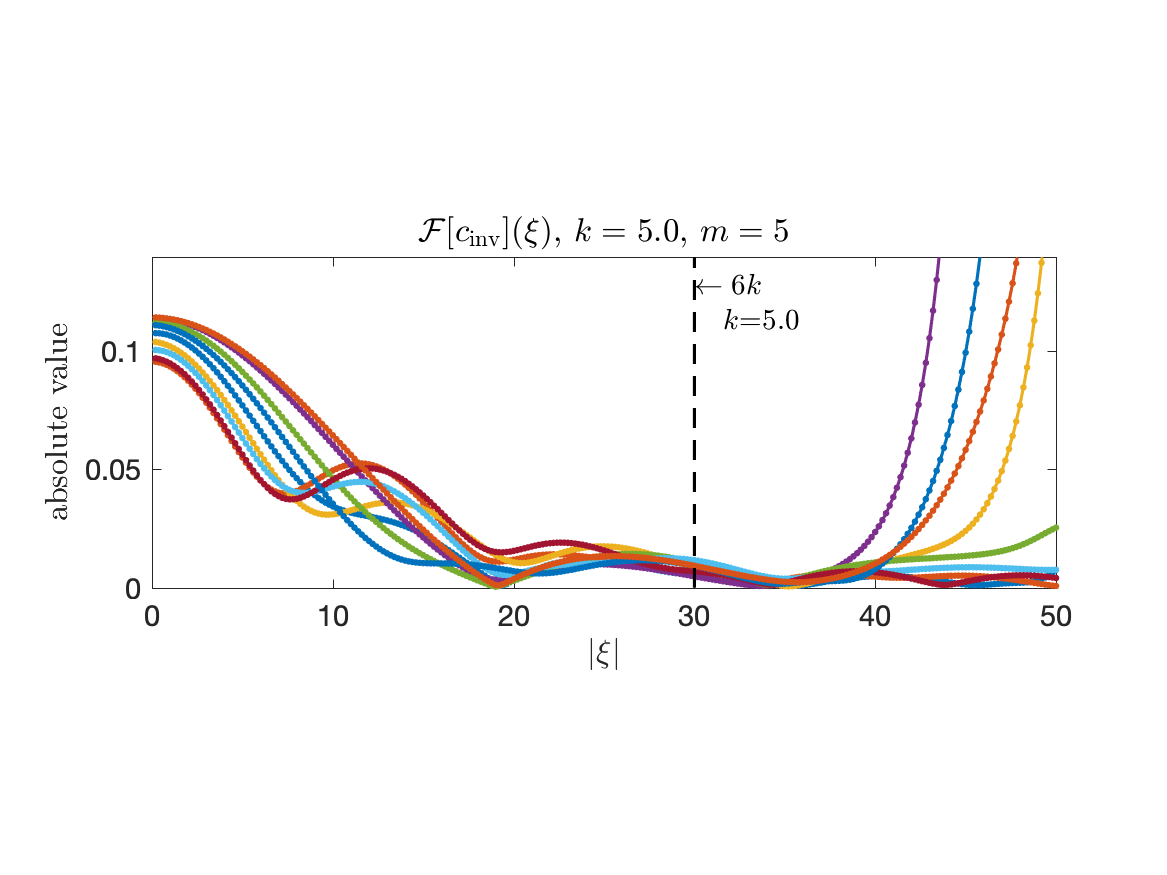
\includegraphics[width=0.54\textwidth,trim=10 60 30 90,clip]{./figs/pwc_5_Fc_0050.png}\\
\,\hfill \textbf{(i)} $k = 10$ \hfill\,\\
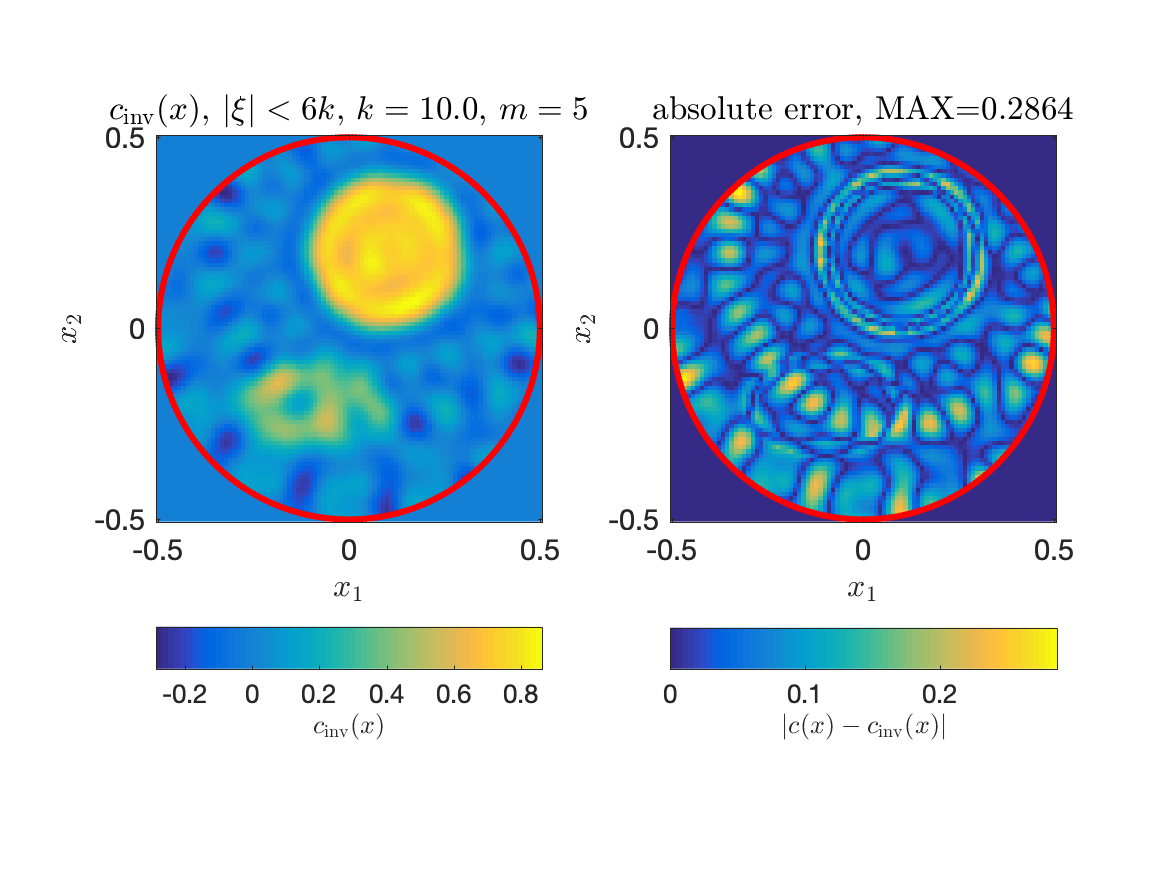
\includegraphics[width=0.45\textwidth,trim=20 60 20 35,clip]{./figs/pwc_5_Ic_0100.png}
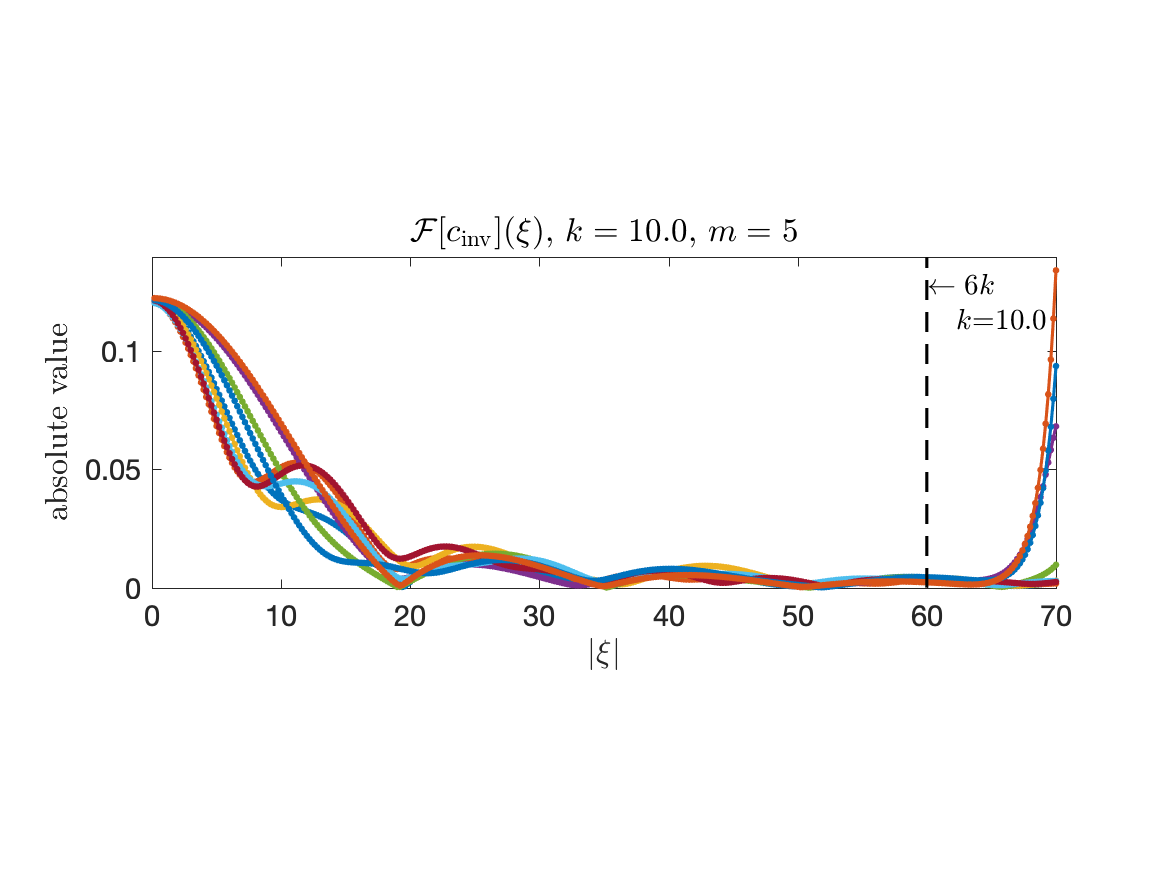
\includegraphics[width=0.54\textwidth,trim=10 60 30 90,clip]{./figs/pwc_5_Fc_0100.png}\\
\,\hfill \textbf{(i)} $k = 15$ \hfill\,\\
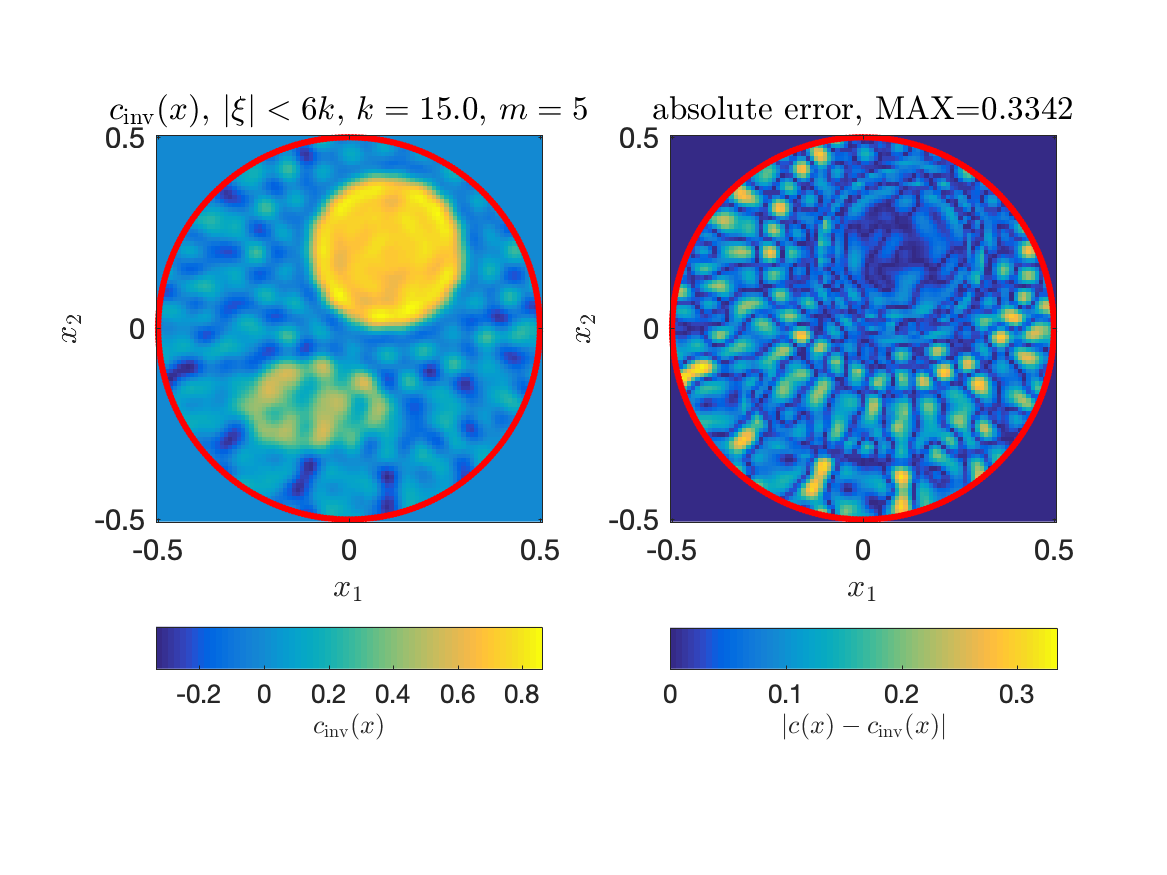
\includegraphics[width=0.45\textwidth,trim=20 60 20 35,clip]{./figs/pwc_5_Ic_0150.png}
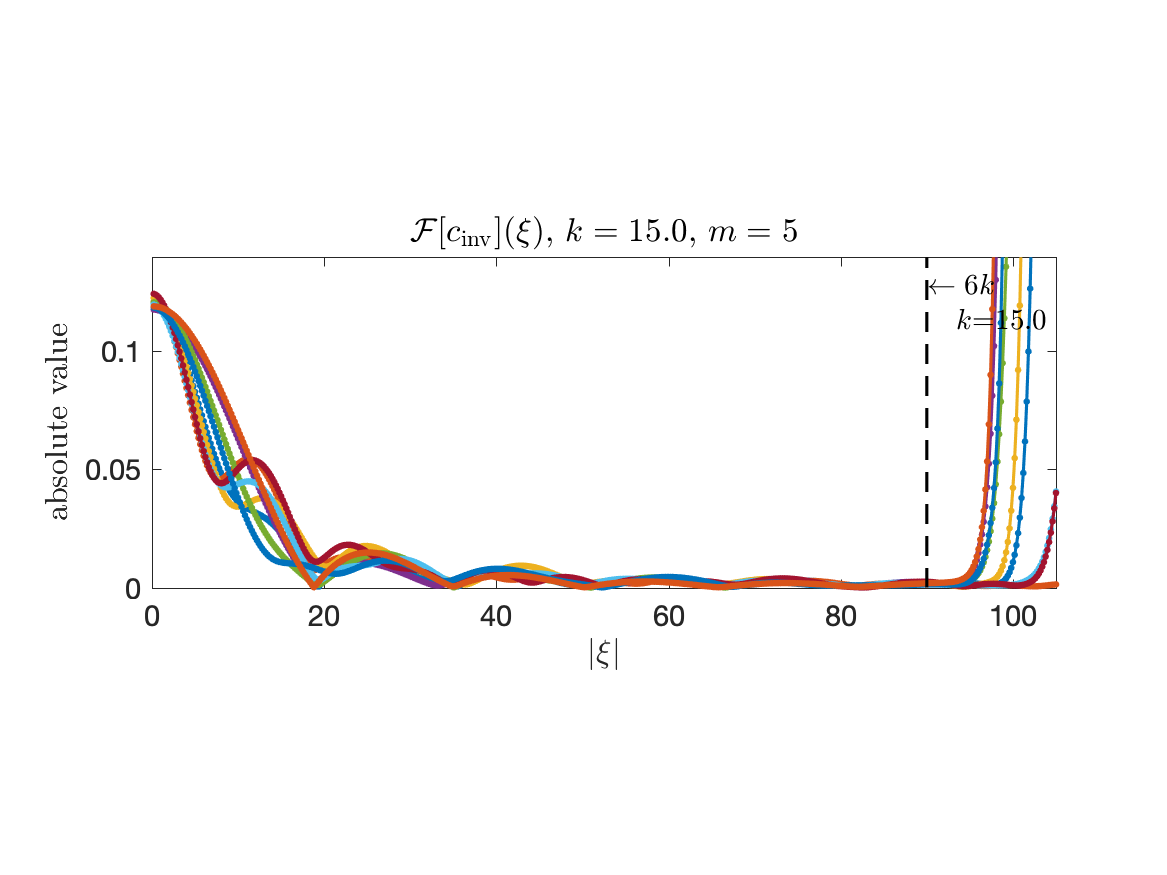
\includegraphics[width=0.54\textwidth,trim=10 60 30 90,clip]{./figs/pwc_5_Fc_0150.png}\\
\caption[算法2:不连续位势的重构结果]{当非线性次数$m=5$,波数\textbf{(i)} $k = 5$,\textbf{(ii)} $k = 10$和\textbf{(iii)} $k = 15$时的重构结果.
第一列:利用频域截断$|\xi| \leq (m+1)k$得到的重构位势函数$c_{\textrm{inv}}(x)$.
第二列:真实位势函数和重构位势函数的角度误差$|c(x) - c_{\textrm{inv}}(x)|$.
第三列:重构位势函数的傅立叶系数的绝对值$\mathcal{F}[c_{\textrm{inv}}](\xi)|$.
}
\label{fig:5_pwc}
\end{figure}

如果多个图形相互独立,并不共用一个图形计数器,那么用 \texttt{minipage} 或者
\texttt{parbox} 就可以,如图~\ref{fig:parallel1} 与图~\ref{fig:parallel2}。

\begin{figure}[H]
  \centering
  \begin{minipage}{0.48\textwidth}
    \centering
    
\includegraphics[height=1.5cm]{./figs/fudan-emblem.pdf}
    \caption{并排第一个图}
    \label{fig:parallel1}
  \end{minipage}\hfill
  \begin{minipage}{0.48\textwidth}
    \centering
    
\includegraphics[height=1.5cm]{./figs/fudan-emblem.pdf}
    \caption{并排第二个图}
    \label{fig:parallel2}
  \end{minipage}
\end{figure}

如果要为共用一个计数器的多个子图添加子图题,建议使用较新的 subcaption 宏包,不建议使用 subfigure 或 subfig 等宏包。

推荐使用 subcaption宏包的 subcaptionbox并排子图,子图题置于子图之下,子图号用 a)、b) 等表示。也可以使用subcaption宏包的 subcaption(放在 minipage中,用法同 caption)。

subcaption 宏包也提供了subfigure和 subtable 环境,如
图~\ref{fig:subfigure}。

\begin{figure}[!htp]
  \centering
  \begin{subfigure}{0.3\textwidth}
    \centering
    
\includegraphics[height=2cm]{./figs/fudan-emblem.pdf}
    \caption{校徽}
  \end{subfigure}
  \hspace{1cm}
  \begin{subfigure}{0.4\textwidth}
    \centering
    
\includegraphics[height=1.5cm]{./figs/fudan-emblem.pdf}
    \caption{校徽。这个图略矮些,subfigure中同一行的子图在顶端对齐。}
  \end{subfigure}
  \caption{包含子图题的范例(使用 subfigure)}
  \label{fig:subfigure}
\end{figure}

\subsection{Tik作图}
以下摘自Hansimov的知乎文章[LaTeX 绘图指南 - 001] TikZ 的简介、资源以及学习方法\footnote{https://zhuanlan.zhihu.com/p/48300815}。

TikZ 是 LaTeX 下的一个(著名的)绘图宏包。TikZ 的德文原文是 TikZ ist kein Zeichenprogramm, 这是一个 "GNU's Not Unix!" 式的递归缩写。翻译成英文就是 TikZ is not a drawing program,中文意思是“TikZ 不是一个绘图程序”。(程序员式冷幽默)

PGF/TikZ 相关的学习资源很多,可以参考这个项目:xiaohanyu/awesome-tikz\footnote{https://github.com/xiaohanyu/awesome-tikz}。基本列出了常见的高质资源,语言大多为英文。此外还有一些重要的资源:

\begin{itemize}
    \item 英文文档:pgfmanual\footnote{http://mirrors.ctan.org/graphics/pgf/base/doc/pgfmanual.pdf}
    \item PGF/TikZ 中文手册(在翻):pgfmanual-zh\footnote{https://github.com/Hansimov/pgfmanual-zh}
    \item 命令大全:VisualTikZ\footnote{http://mirrors.ctan.org/info/visualtikz/VisualTikZ.pdf}
     \item 各种样例:TikZ and PGF examples\footnote{http://www.texample.net/tikz/examples/all/}
     \item TeX 社区:Questions tagged [tikz-pgf]\footnote{https://tex.stackexchange.com/questions/tagged/tikz-pgf}
\end{itemize}

下面是来自于邹森博士论文中的一个样例。
\begin{figure}[H]
\centering
%----------------------%
% original, STYLE 1
\begin{tikzpicture}[>=latex,scale=1.0]
\draw[rounded corners=8,dashed,fill=gray!15!white]
 (0.6,-0.8) rectangle (2.6,0.8) node at ++(-0.3,-0.3) {$\Omega$};
\node  (f) at (0,0) {$f$};
\node  (u) at (2,0) {$u$};
\node (du) at (4,0) {$\partial_{\nu} u$};
\draw[->,thick,blue] (f) -- node[above] {$c$}  (u) node[pos=0.5,below] {\footnotesize$(I)$};
\draw[->,thick] (u) -- (du) node[pos=0.5,below] {\footnotesize$\partial_{\nu}$};
\draw[rounded corners=15,->,thick,blue] (f) |- (2,1.2) node[above] {$\Lambda_{c}$} -| (du);
\node at (2,-1.3) {\textbf{(i)} 原始问题};
\end{tikzpicture}%\\
%----------------------%
% linearized
\hspace{4ex}
\begin{tikzpicture}[>=latex,scale=1.0]
\draw[rounded corners=8,dashed,fill=gray!15!white]
 (0.5,-0.8) rectangle (4.6,0.8) node at ++(-0.3,-0.3) {$\Omega$};
\node   (f) at (0,0) {$f$};
\node  (u0) at (2,0) {$u^{(0)}$};
\node  (u1) at (4,0) {$u^{(1)}$};
\node (du1) at (6,0) {$\partial_{\nu} u^{(1)}$};
\draw[->,thick]  (f) --  (u0) node[pos=0.5,below] {\footnotesize$(I_{0})$};
\draw[->,thick,blue] (u0) -- node[above] {$c$}  (u1) node[pos=0.5,below] {\footnotesize$(I_{1})$};
\draw[->,thick] (u1) -- (du1) node[pos=0.5,below] {\footnotesize$\partial_{\nu}$};
\draw[rounded corners=15,->,thick,blue] (f) |- (3,1.2) node[above] {$\Lambda'_{c}$} -| (du1);
\node at (3,-1.3) {\textbf{(ii)} 线性化系统};
\end{tikzpicture}\\
%----------------------%
% PIE type
\vspace{1ex}
\begin{tikzpicture}[>=latex,scale=1.0]
\draw[rounded corners=8,dashed,fill=gray!15!white]
 (0.5,-1) rectangle (6.6,1) node at ++(-0.3,-0.3) {$\Omega$};
\node   (f) at (0,0) {$f_{j}$};
\draw[rounded corners=2,red] (-0.5,0.7) rectangle (2.45,-0.7) node at ++(-0.4,0.2) {\tiny$j \in S$};
\node  (u0) at (2,0) {$u_{j}^{(0)}$};
\node  (v0) at (4,0) {$u_{S}^{(0)}$};
\node  (v1) at (6,0) {$u_{S}^{(1)}$};
\node (dv1) at (8,0) {$\partial_{\nu} u_{S}^{(1)}$};
\draw[->,thick]  (f) --  (u0) node[pos=0.5,below] {\footnotesize$(I_{0})$};
\draw[->,thick,red] (u0) --  (v0) node[pos=0.5,below] {\footnotesize$\sum\limits_{j \in S}$};
\draw[->,thick,blue] (v0) -- node[above] {$c$}  (v1) node[pos=0.5,below] {\footnotesize$(I_{S}^{(1)})$};
\draw[->,thick] (v1) -- (dv1) node[pos=0.5,below] {\footnotesize$\partial_{\nu}$};
\draw[rounded corners=2] (-0.7,1.3) rectangle (8.7,-1.3) node at ++(-0.4,0.2) {\tiny$S \subseteq U$};
\draw[rounded corners=15,->,thick,blue] (f)++(0,0.7) |- (4,1.6) node[above] {$\Lambda'_{c}$} -| (dv1);
\node at (4,-1.8) {\textbf{(iii)} PIE型线性化系统};
\end{tikzpicture}
%----------------------%
\caption[Alessandrini等式示意图]{三种Alessandrini型等式的对比图示}
\label{fig:identity}
\end{figure}


\section{表格}

\subsection{基本表格}

编排表格应简单明了,表达一致,明晰易懂,表文呼应、内容一致。表题置于表上。

表格的编排建议采用国际通行的三线表\footnote{三线表,以其形式简洁、功能分明、阅读
方便而在科技论文中被推荐使用。三线表通常只有 3 条线,即顶线、底线和栏目线,没有竖线。}。三线表可以使用 booktabs 提供的 toprule、midrule 和bottomrule。它们与 longtable能很好的配合使用。

\begin{table}[!hpt]
  \caption[一个颇为标准的三线表]{一个颇为标准的三线表\footnotemark}
  \label{tab:firstone}
  \centering
  \begin{tabular}{@{}llr@{}} \toprule
    \multicolumn{2}{c}{Item} \\ \cmidrule(r){1-2}
    Animal & Description & Price (\$)\\ \midrule
    Gnat  & per gram  & 13.65 \\
          & each      & 0.01 \\
    Gnu   & stuffed   & 92.50 \\
    Emu   & stuffed   & 33.33 \\
    Armadillo & frozen & 8.99 \\ \bottomrule
  \end{tabular}
\end{table}
\subsection{复杂表格}

我们经常会在表格下方标注数据来源,或者对表格里面的条目进行解释。可以用threeparttable实现带有脚注的表格,如表~\ref{tab:footnote}。

\begin{table}[!htpb]
  \bicaption{一个带有脚注的表格的例子}{A Table with footnotes}
  \label{tab:footnote}
  \centering
  \begin{threeparttable}[b]
     \begin{tabular}{ccccccc}
      \toprule
      \multirow{2}*{total} & \multicolumn{2}{c}{20\tnote{a}} & \multicolumn{2}{c}{40} & \multicolumn{2}{c}{60} \\
      \cmidrule(lr){2-3}\cmidrule(lr){4-5}\cmidrule(lr){6-7}
      & www & \multicolumn{1}{c}{k} & www & k & www & k \\ % 使用说明符 d 的列会自动进入数学模式,使用 \multicolumn 对文字表头做特殊处理
      \midrule
      & $\underset{(2.12)}{4.22}$ & 120.0140\tnote{b} & 333.15 & 0.0411 & 444.99 & 0.1387 \\
      & 168.6123 & 10.86 & 255.37 & 0.0353 & 376.14 & 0.1058 \\
      & 6.761    & 0.007 & 235.37 & 0.0267 & 348.66 & 0.1010 \\
      \bottomrule
    \end{tabular}
    \begin{tablenotes}
    \item [a] the first note.
    \item [b] the second note.
    \end{tablenotes}
  \end{threeparttable}
\end{table}

如某个表需要转页接排,可以用longtable实现。接排时表题省略,表头应重复书
写,并在右上方写“续表 xx”,如表~\ref{tab:performance}。

\begin{ThreePartTable}
  \begin{TableNotes}
    \item[a] 一个脚注
    \item[b] 另一个脚注
  \end{TableNotes}
  \begin{longtable}[c]{c*{6}{r}}
    \bicaption{实验数据}{Experimental data}
    \label{tab:performance} \\
    \toprule
    测试程序 & \multicolumn{1}{c}{正常运行} & \multicolumn{1}{c}{同步}
      & \multicolumn{1}{c}{检查点} & \multicolumn{1}{c}{卷回恢复}
      & \multicolumn{1}{c}{进程迁移} & \multicolumn{1}{c}{检查点} \\
    & \multicolumn{1}{c}{时间 (s)} & \multicolumn{1}{c}{时间 (s)}
      & \multicolumn{1}{c}{时间 (s)} & \multicolumn{1}{c}{时间 (s)}
      & \multicolumn{1}{c}{时间 (s)} &  文件(KB)\\
    \midrule
    \endfirsthead
    \multicolumn{7}{l}{\textbf{续表~\thetable}} \\
    % 英语论文:\multicolumn{7}{r}{\textbf{Table~\thetable~(continued)}} \\
    \toprule
    测试程序 & \multicolumn{1}{c}{正常运行} & \multicolumn{1}{c}{同步}
      & \multicolumn{1}{c}{检查点} & \multicolumn{1}{c}{卷回恢复}
      & \multicolumn{1}{c}{进程迁移} & \multicolumn{1}{c}{检查点} \\
    & \multicolumn{1}{c}{时间 (s)} & \multicolumn{1}{c}{时间 (s)}
      & \multicolumn{1}{c}{时间 (s)} & \multicolumn{1}{c}{时间 (s)}
      & \multicolumn{1}{c}{时间 (s)}&  文件(KB)\\
    \midrule
    \endhead
    \hline
    \multicolumn{7}{r}{续下页}
    \endfoot
    \insertTableNotes
    \endlastfoot
    CG.A.2 & 23.05 & 0.002 & 0.116 & 0.035 & 0.589 & 32491 \\
    CG.A.4 & 15.06 & 0.003 & 0.067 & 0.021 & 0.351 & 18211 \\
    CG.A.8 & 13.38 & 0.004 & 0.072 & 0.023 & 0.210 & 9890 \\
    CG.B.2 & 867.45 & 0.002 & 0.864 & 0.232 & 3.256 & 228562 \\
    CG.B.4 & 501.61 & 0.003 & 0.438 & 0.136 & 2.075 & 123862 \\
    CG.B.8 & 384.65 & 0.004 & 0.457 & 0.108 & 1.235 & 63777 \\
    MG.A.2 & 112.27 & 0.002 & 0.846 & 0.237 & 3.930 & 236473 \\
    MG.A.4 & 59.84 & 0.003 & 0.442 & 0.128 & 2.070 & 123875 \\
    MG.A.8 & 31.38 & 0.003 & 0.476 & 0.114 & 1.041 & 60627 \\
    MG.B.2 & 526.28 & 0.002 & 0.821 & 0.238 & 4.176 & 236635 \\
    MG.B.4 & 280.11 & 0.003 & 0.432 & 0.130 & 1.706 & 123793 \\
    MG.B.8 & 148.29 & 0.003 & 0.442 & 0.116 & 0.893 & 60600 \\
    LU.A.2 & 2116.54 & 0.002 & 0.110 & 0.030 & 0.532 & 28754 \\
    LU.A.4 & 1102.50 & 0.002 & 0.069 & 0.017 & 0.255 & 14915 \\
    LU.A.8 & 574.47 & 0.003 & 0.067 & 0.016 & 0.192 & 8655 \\
    LU.B.2 & 9712.87 & 0.002 & 0.357 & 0.104 & 1.734 & 101975 \\
    LU.B.4 & 4757.80 & 0.003 & 0.190 & 0.056 & 0.808 & 53522 \\
    LU.B.8 & 2444.05 & 0.004 & 0.222 & 0.057 & 0.548 & 30134 \\
    EP.A.2 & 123.81 & 0.002 & 0.010 & 0.003 & 0.074 & 1834 \\
    EP.A.4 & 61.92 & 0.003 & 0.011 & 0.004 & 0.073 & 1743 \\
    EP.A.8 & 31.06 & 0.004 & 0.017 & 0.005 & 0.073 & 1661 \\
    EP.B.2 & 495.49 & 0.001 & 0.009 & 0.003 & 0.196 & 2011 \\
    EP.B.4 & 247.69 & 0.002 & 0.012 & 0.004 & 0.122 & 1663 \\
    EP.B.8 & 126.74 & 0.003 & 0.017 & 0.005 & 0.083 & 1656 \\
    SP.A.2 & 123.81 & 0.002 & 0.010 & 0.003 & 0.074 & 1854 \\
    SP.A.4 & 51.92 & 0.003 & 0.011 & 0.004 & 0.073 & 1543 \\
    SP.A.8 & 31.06 & 0.004 & 0.017 & 0.005 & 0.073 & 1671 \\
    SP.B.2 & 495.49 & 0.001 & 0.009 & 0.003 & 0.196 & 2411 \\
    SP.B.4 \tnote{a} & 247.69 & 0.002 & 0.014 & 0.006 & 0.152 & 2653 \\
    SP.B.8 \tnote{b} & 126.74 & 0.003 & 0.017 & 0.005 & 0.082 & 1755 \\
    \bottomrule
  \end{longtable}
\end{ThreePartTable}

\section{算法环境}

算法环境可以使用 agorithms宏包或者较新的algorithm2e实现。
算法~\ref{algo:algorithm} 是一个使用algorithm2e的例子。关于排版算法环境
的具体方法,请阅读相关宏包的官方文档。

\begin{algorithm}[htb]
  \caption{算法示例}
  \label{algo:algorithm}
  \small
  \SetAlgoLined
  \KwData{this text}
  \KwResult{how to write algorithm with \LaTeXe }

  initialization\;
  \While{not at end of this document}{
    read current\;
    \eIf{understand}{
      go to next section\;
      current section becomes this one\;
    }{
      go back to the beginning of current section\;
    }
  }
\end{algorithm}

同样可以考虑以如下表格的形式实现。
\begin{table}[H] 
\centering
\begin{tabular}{p{\textwidth}}
\toprule
\textbf{算法1:3维情况下部分边界观测反问题$\lambda_c\rightarrow c$的神经网络结构}  \\%
\midrule
\textbf{输入:} %
$\lambda\in\mathbb{R}^{N_{m_1}\times N_{m_2}\times N_{h_1}\times N_{h_2}}$,参数$channel,N_{z},w,n_{cnn}$;
\textbf{输出:} %
$c\in \mathbb{R}^{N_x\times N_y\times N_y}$. \\[-15pt]%
\begin{enumerate}[1:]
  \item 将$\lambda_c$的后两个维度向量化,形成一个三维张量,记为$\lambda$;
  \item $\tilde{\lambda}_{\hat{h}}\leftarrow\texttt{Encoding3d}[channel](\lambda)$; %
  \item  $\tilde{c}_{\hat{z}_3}\leftarrow\texttt{BCR-Net2d}(\tilde{\lambda}_{\hat{h}}) $; %
  \item $\bar{c}\leftarrow\texttt{Decoding3d}[N_z](\tilde{c}_{\hat{z_3}})$;%
  \item $c\leftarrow\texttt{CNN3d}[w,n_{cnn}](\bar{c})$;%
  \item 返回 $c$ %
\end{enumerate} \\%
\bottomrule
\end{tabular}
\caption*{算法 1: 线性薛定谔位势反问题的部分边界观测问题的神经网络结构\parencite{FY2020}}
\end{table}







% 附录
\appendix
% !TeX root = ../main.tex
\chapter{代码}
\section{代码环境}
我们可以在论文中插入算法,但是不建议插入大段的代码。如果确实需要插入代码,建议使用listings宏包。
\begin{codeblock}[language=MATLAB]
x = [1, 2, 3, 4, 5]';
y = [2, 4, 6, 8, 10]';
theta = [0; 0];
learning_rate = 0.01;
num_iterations = 100;

for iter = 1:num_iterations
    idx = randi(length(x));
    x_i = x(idx);
    y_i = y(idx);
    grad = [x_i, 1]' * (theta' * [x_i, 1]' - y_i);
    theta = theta - learning_rate * grad;
end
fprintf('theta1: %f, theta0: %f\n', theta(1), theta(2));
\end{codeblock}



% 结尾部分
\backmatter

% 用于盲审的论文需隐去致谢、发表论文、科研成果、



% 打印参考文献列表
\printbibliography
\renewcommand{\bibname}{参考文献}

\begin{acknowledgements}
  致谢
\end{acknowledgements}


% 发表论文及科研成果
\chapter*{攻读学位期间研究成果}
\addcontentsline{toc}{chapter}{\normalfont \sffamily 攻读学位期间研究成果}
\begin{enumerate}
\item Authors. Title. \textit{Journal Name}, xx(x),2022: xxx–xxx,
\item Authors. Title. Submitted to \textit{Journal Name}, arXiv: xxxxxx, 2022,
\end{enumerate}
\end{document}





